\section{Recta tangente a una curva}
Sea $C \subset \mathbb{R}^m$ la curva de ecuación $X= \vec{g}(t)$ con $t\in I$. En todo punto simple 
y regular $\vec{A} = \vec{g}(t) \in C$, la curva adminte recta tangente de ecuación:

$$
\vec{X} = \vec{A} + u \vec{g}  \, ' (t_0)  \, u \in \mathbb{R}
$$

\begin{figure}[H] 
    \centering    
    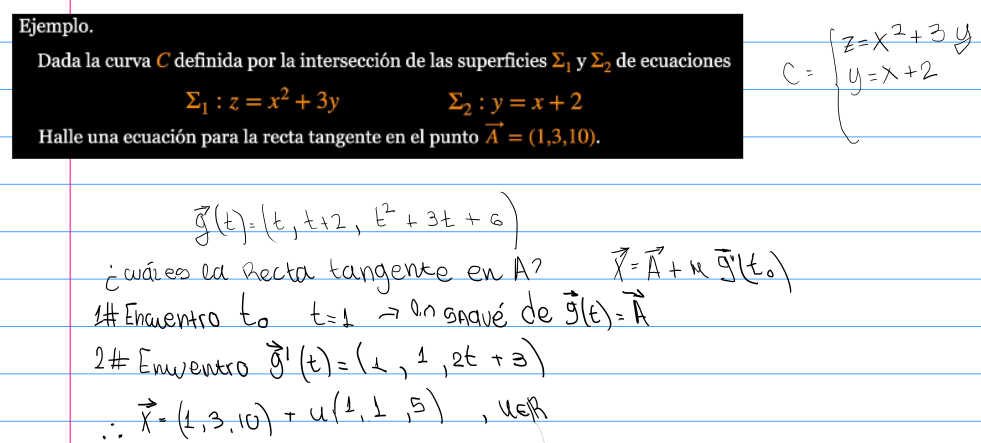
\includegraphics[width=0.8\textwidth]{img/ej-rec-tan.png}
    \label{fig:ej-rec-tans}
\end{figure}

\subsection{Curva plana en $\mathbb{R}^2$ - Recta normal} 
\label{sec:recta-tangente}
Si $A = \vec{g}(t_0)$ es un punto simple y regular de $C$ y si la ecuación
de la recta tangente $r_0$ en $A$ la escribimos:
$$
\vec{X} = \vec{A} + u \,  \vec{g}  \, ' (t_0)  \, , u \in \mathbb{R}
$$
Entonces, obtenemos una ecuación para la recta normal $n_0$ en $A$:
$$
\vec{X} = \vec{A} + v   \, \vec{g}  \, ' (t_0)_{\perp}  \, , v \in \mathbb{R}
$$
Donde $\vec{g}  \, ' (t_0)_{\perp} \, . \, \vec{g}  \, ' (t_0) = 0$, es decir,
$\vec{g} \, ' (t_0)_{\perp}$ es un vector perpendicular y no nulo a $\vec{g}  \, ' (t_0)$.
\subsection{Curva plana en $\mathbb{R}^3$ - Plano normal}
Dada las condiciones de \ref{sec:recta-tangente}, el plano normal $\pi_0$ en $A$ tiene por ecuación:
$$
(\vec{X} - \vec{A}) \, . \, \vec{g}  \, ' (t_0) = 0
$$

\begin{figure}[H] 
    \centering    
    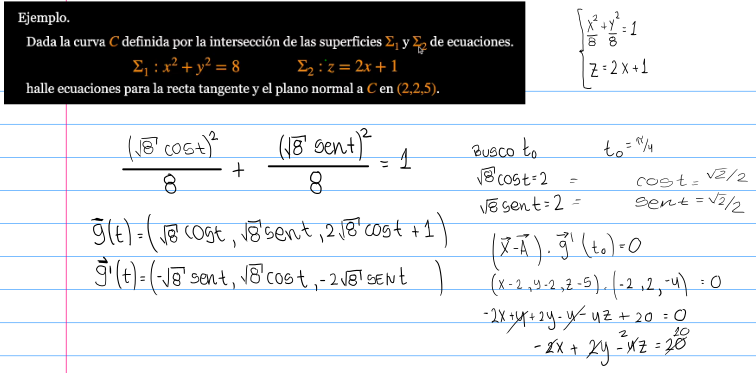
\includegraphics[width=0.8\textwidth]{img/ej-rec-tan2.png}
    \label{fig:ej-rec-tan2}
\end{figure}
